%%%%%%%%%%%%%%%%%%%%%%%%%%
% Statistical Programming Languages  
% 
% Dr Alla 
% Humboldt Universitat zu Berlin
% 15 March 2019
%%%%%%%%%%%%%%%%%%%%%%%%%%


\documentclass[11pt]{article}
\usepackage[margin=1.2in]{geometry}
\usepackage[toc,page]{appendix}
\usepackage{graphicx}
\usepackage{natbib}
\usepackage{lipsum}
\usepackage{caption}
\usepackage{pdflscape}
\usepackage[utf8]{inputenc}
\usepackage[english]{babel}
\usepackage[svgnames]{xcolor}
\usepackage{listings}
\lstset{language=R,
    basicstyle=\small\ttfamily,
    stringstyle=\color{DarkGreen},
    otherkeywords={0,1,2,3,4,5,6,7,8,9},
    morekeywords={TRUE,FALSE},
    deletekeywords={data,frame,length,as,character},
    keywordstyle=\color{blue},
    commentstyle=\color{DarkGreen},
}


\begin{document}

\captionsetup[figure]{margin=1.5cm,font=small,labelfont={bf},name={Figure},labelsep=colon,textfont={it}}
\captionsetup[table]{margin=1.5cm,font=small,labelfont={bf},name={Table},labelsep=colon,textfont={it}}
\setlipsumdefault{1}


\begin{titlepage}


% -------------------------------------------------------------------
% You need to edit the details here
% -------------------------------------------------------------------

\begin{center}
{\LARGE Humboldt Universitat zu Berlin}\\[1.5cm]
\linespread{1.2}\huge {\bfseries Title}\\[1.5cm]
\linespread{1}
{\Large Your Name}\\[1cm]
{\large \emph{Supervisor:} Supervisor's Name}\\[1cm] % if applicable
\large A report submitted in partial fulfilment of the requirements\\ for the degree of ???? in Computer Science\\[0.3cm] 
\textit{in the}\\[0.3cm]
Department of Computer Science\\[2cm]
\today
\end{center}

\end{titlepage}


% -------------------------------------------------------------------
% Declaration
% -------------------------------------------------------------------

\newpage

\tableofcontents

\newpage

\listoffigures

\newpage

\listoftables


% -------------------------------------------------------------------
% Main sections (as required)
% -------------------------------------------------------------------

\newpage



\section{Motivation}

Qi  Go girl go !


\section{Methodology}
The concept of "livability" lacks clearly defined theoretical framework in the literature \citep{giap2014new}. This complex measure is often used in empirical studies, to rank and compare different geographical areas in terms of the "quality of life" or "well-being" offered to their inhabitants. The last three decades of research on happiness has shown that the well-being should be measured with social, economical and also subjective to the given group set of indicators \citep{diener1997measuring}. In cities, livability is often defined in terms of greenery, security, economic stability, infrastructure and night life \citep{ unit2011liveanomics}.  
Number of city rankings have been published by institutions such as C40, the World Economic Forum \citep{Okulicz-Kozaryn2013}. However, for the purpose of this study, each of the existing methodologies required its adaptation to the city district level.  

\subsection{Liveability Standards in Cities}

The "Methodology for Collection and Computation of Liveability Standards in Cities" developed by Government of India breaks down the Index calculation 
to its primary components \citep{methodology}.
The methodology divides the liveability standards indicators in the cities into four pillars: 1. Institutional, 2. Social, 3. Economic and 4. Physical. 
For each pillar "Sub-Indexes" were calculated and weighted respectively with 25\%, 25\%, 5\% and 45\% towards final Index. To calculate the sub-Indexes, respective normalized indicators were added.   

A total of 79 indicators are used for the calculation of the Liveability Index. To eliminate the issue of difference in units and scales, each of the indicators was normalized using the equation \ref{eq:1} (variable has positive impact on the Index) or equation \ref{eq:2}  (negative impact).      
\begin{equation}
I_i^+ = \frac{I_i- I_{min}}{I_{max}- I_{min}}
\label{eq:1}
\end{equation}
 
 \begin{equation}
I_i^- = \frac{I_{max}- I_i}{I_{max}- I_{min}}
\label{eq:2}
\end{equation}

\subsection{Adaptation of the methodology to districts of Berlin}
 
The Berlin Districts Liveability Index adapts the described in the section 1.2.1 methodology for the purpose of district comparison. Taking into account current socio-economic situation and potential measurable differences between districts, the Index is based on four pillars with following the argumentation:
\\ 
\textbf{1. Physical}: Berlin is facing rapid population increase and shortage of housing \citep{Schultheis.2019}. It becomes increasingly difficult to find affordable housing in districts with good infrastructure. Nonetheless, availability of housing is more pressing then the infrastructure. 
\\ 
\textbf{2.Social}: Berlin is well known for night life, which brought more than €1.5 billion to the city in 2018 \citep{Local.2019}. Besides "cool" cultural side, other indicators such as education, health, safety and social support need to be considered. This is the biggest pillar of the index with 16 indicators.
\\
\textbf{3. Economic}: Rapidly growing start-up scene in Berlin and its reputation of being "Silicon Valley of Europe" brings more and more business to the city \citep{cooke2015skill}. Consequently, there is a big competition between districts to attract big players planning to move here (e.g. Google) \citep{Kuhn.2019}. 
\\
\textbf{4. Environmental}: Due to the growing air pollution threat in Berlin \citep{tagesspiegel.2019} and concerns regarding the environmental health in the cities, the Institutional Category of the Index has been replaced by Environmental. The environmental health and greenery of the districts is considered.\\
The methodology for the Berlin District Liveability Index is illustrated by Figure \ref{fig:meth}. Complete list of the indicators and their description can be found in Annex A. 

\begin{figure}[h]

\centering
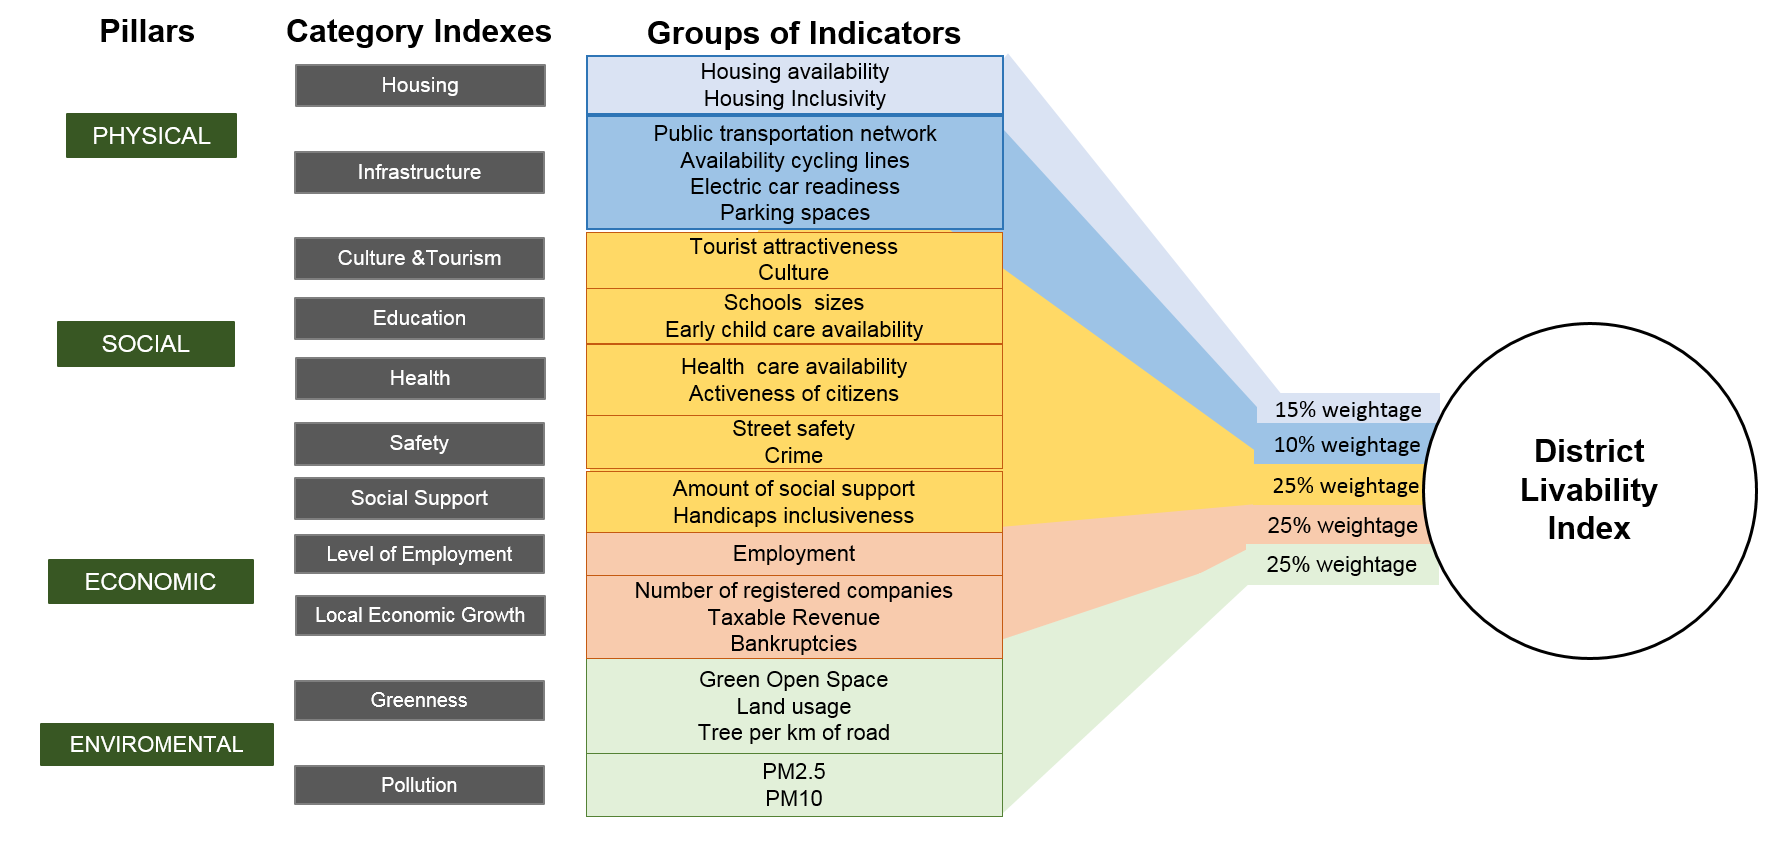
\includegraphics[scale=0.35]{images/Methodology.png}
\caption{Berlin Districts Livability Index Calculation Methodology }
\label{fig:meth}
\end{figure}



\newpage
\section{Data Preparation}

According to seminal research by \cite{Reference1}, lorem ipsum dolor sit amet.  However, this result was already known in the 1990s \citep{Reference2,Reference3}.  % Note the use of \cite{} and \citep{}


\section{A Section that Contains Some Maths}

\lipsum  % Replace with your text
 
\begin{equation}
M = \frac{1}{T}\sum_{t=1}^{T} e(t) / \max_{t}[e(t)]
\label{eq:equation}
\end{equation}

\lipsum  % Replace with your text

This is shown in Equation \ref{eq:equation} and is repeated here $M = \frac{1}{T}\sum_{t=1}^{T} e(t) / \max_{t}[e(t)]$.


\section{A Section that Contains a Figure}

\lipsum  % Replace with your text

\begin{figure}[ht]
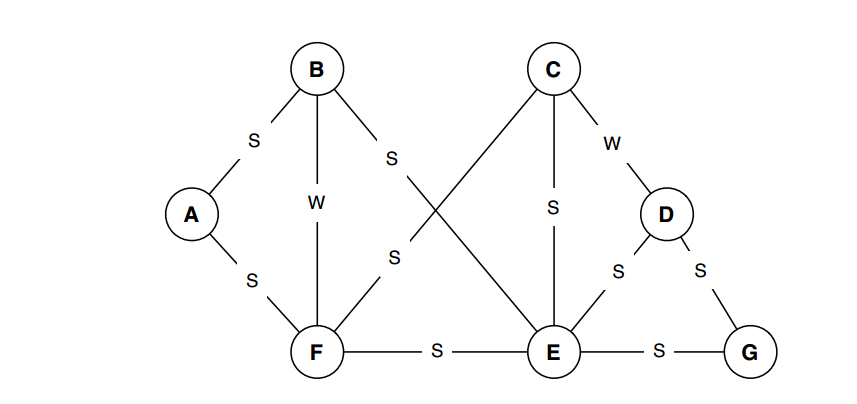
\includegraphics[width=15cm]{figures/figure1.png}
\caption{A simple figure in \LaTeX. Reproduced from http://tinyurl.com/nqtrlj5 with the permission of the copyright owner.}
\label{fig:graph}
\end{figure}

\lipsum  % Replace with your text

See Figure \ref{fig:graph}.


\section{A Section that Contains a Table}

\lipsum  % Replace with your text

\begin{table}[ht]
\center
\begin{tabular}{cc|c}
A & B & A XOR B\\
\hline
0 & 0 & 0\\
0 & 1 & 1\\
1 & 0 & 1\\
1 & 1 & 0\\
\end{tabular}
\caption{A simple table in \LaTeX.}
\label{tab:xor}
\end{table}

\lipsum  % Replace with your text

This is shown in Table \ref{tab:xor}.


\section{Summary}

\lipsum  % Replace with your text

\newpage
\section{Liveability Index}

The following chapter will used the final Data Set to calculate the Liveavility Index for each district of Berlin. Firstly, code used for indicators calculation and their normalization will be explained. Secondly, Sub- and Total Indexes will be calculated and thirdly, the results will presented and discussed .

\subsection{Indicators}
\subsubsection{Calculating Indicators}
To calculate Berlin Districts Liveability Index the total of 33 indicators have been considered. To be able to compare the indicators between districts, the relative values (rather then the absolute) of the variables had to be consider. For this purpose, most of the variables have been converted to per capita or per Hectare terms. In the code two functions have been written:

\begin{lstlisting}
PerCapita = function(x){
    # Function divides the data per number of 
    # inhabitants of given district to  obtain per capita value 
    #Args: 
    #    x: the column of which the data should decided 
    #      per number of citizens
    # Returns:
    # The vector of data x divided per number of inhabitants
    # of given district
  x/lvbInDt$Population
}

PerHa = function(x){
    # Function divides the data by size in ha of given
    # district to obtain per ha value
    #Args: 
    #    x: the column of which the data should 
    #    divided by size of the district
    # Returns:
    # The vector of data x divided by size of the district in ha
  x/lvbInDt$Size
}

\end{lstlisting}

The list of the indicators and their description may be found in Annex A. The two functions has been applied to following indicators:
 \begin{table}[ht]
\centering
\begin{tabular}{rll}
  \hline
 Method & Indicator \\ 
  \hline
 Per Capita & lvSpc, hsAv, prkSp, trs, doc, trf, socHl \\ 
 Per Ha & \parbox[t]{8cm}{dns, trnDn, bkLN, sprCl, crChr,res, strCr, grSp}  \\ 
 Other & \parbox[t]{8cm}{hsAl, htlOc, std, grdSz, chU3, chU6, actSn, actJn,crm, dsb, emp, comp trRv, bnk, agrRe, tr, pm10, pm25} \\ 
   \hline
\caption{Methods for calculating Indicators}
\end{tabular}
\end{table}
If the functions has not be been applied, it means that the variable was already expressed in the relative value or that absolute value was reasonable indicator to be used ex. total taxable revenue of the companies in the given district. For more details see Annex A and 94:134 lines of code in Quantlet 3 - "SPL-Berlin-DstLivIndex-Calc".  

\subsection{Normalizing Indicators}

\section{Sub-Indexes and Total Liveability Index}

\subsection{Sub-Indexes Calculation}

\subsection{Total Liveability Index Calculation}



\section{Results and Interpretation}


\chapter{Results}

\section{Experiment 1}

\lipsum  
% latex table generated in R 3.4.3 by xtable 1.8-3 package
% 
\begin{tabular}{rlrrrrr}
  \hline
 & District & Phy1In & Phy2In & SocIn & EcoIn & EnvIn \\ 
  \hline
1 & Charlottenburg-Wilmersdorf & 3.13 & 2.19 & 8.16 & 2.61 & 2.47 \\ 
  2 & Friedrichshain-Kreuzberg & 1.68 & 2.81 & 8.10 & 2.25 & 1.37 \\ 
  3 & Lichtenberg & 2.20 & 1.38 & 7.58 & 0.58 & 2.79 \\ 
  4 & Marzahn-Hellersdorf & 2.04 & 1.19 & 5.50 & 0.21 & 2.41 \\ 
  5 & Mitte & 1.69 & 3.81 & 8.51 & 3.47 & 1.47 \\ 
  6 & Neukolln & 1.24 & 1.39 & 5.39 & 1.01 & 2.03 \\ 
  7 & Pankow & 2.45 & 1.16 & 7.46 & 2.75 & 2.63 \\ 
  8 & Reinickendorf & 2.13 & 1.01 & 5.69 & 0.42 & 3.24 \\ 
  9 & Spandau & 1.93 & 0.48 & 5.86 & 0.06 & 2.85 \\ 
  10 & Steglitz-Zehlendorf & 2.68 & 0.68 & 6.56 & 1.49 & 2.61 \\ 
  11 & Tempelhof-Schoneberg & 1.87 & 1.46 & 7.10 & 2.03 & 1.83 \\ 
  12 & Treptow-Kopenick & 2.76 & 0.69 & 4.91 & 1.07 & 1.70 \\ 
  13 & Max Score & 4.00 & 4.00 & 16.00 & 4.00 & 5.00 \\ 
   \hline
\end{tabular}


\section{Experiment 2}

\lipsum  % Replace with your text

\chapter{Discussion}

\lipsum  

\chapter{Conclusions}

\lipsum  % Replace with your text



% -------------------------------------------------------------------
% Bibliography
% -------------------------------------------------------------------

\bibliographystyle{agsm} 
\bibliography{mybibliography} 


% -------------------------------------------------------------------
% Appendices
% -------------------------------------------------------------------
\begin{appendices}
\chapter{Table of Indicators}
\lipsum[1-3]
\begin{landscape}

\section{Landscape page}
 \begin{table}[ht]
\centering
\resizebox{\textwidth}{!}{\begin{tabular}{rlrrrrrrr}
  \hline
 & Pilar & Sub.Index & Weight. & Category. & Indicators & Name.of.the.Indicator.in.the.code & Value & Type.of.Indicator & Unit \\ 
  \hline
1 & Physical & 1. Housing  & 0.15 & 1.1 Housing avaiability  & 1.1.1  Living space  & lvSpc & Living space per capita & indDt = data.frame(lvSpc = PerCapita(lvbInDt\$SpacePC),  \# Calc. liv space/cap. & m2/person \\ 
  2 &  &  &  &  & 1.1.2. Housing avaiable  & hsAv & Number of flats,  District size & hsAv  = PerCapita(lvbInDt\$Flats),  \# Calc. nr of flats/cap. & nr/ha \\ 
  3 &  &  &  &  & 1.1.3 Density of population & dns & Population, District Size & dns   = PerHa(lvbInDt\$Population),  \# Calc. population per ha & nr/ha \\ 
  4 &  &  &  & 1.2 Housing Inclusivness & 1.2.1. Housing Benefits & hsAl & Housing allowance households & hsAl  = lvbInDt\$Hausehold, \# Choose hous. all. & total number \\ 
  5 &  &  2. Infrastracture & 0.10 & 2.1 Avaiability of Public Transportation Network & 2.1.1 Density of  Public Transportation Network & trnDn & Number of Stops & trnDn = PerHa(lvbInDt\$Transport),  \# Calc. den. of pub. trans. & nr/ha \\ 
  6 &  &  &  & 2.2 Cycling lines avaiability & 2.2.1 Lenthg of  cycling lines & bkLn & Meters of cycling lines avaiable  & bkLn  = PerHa(lvbInDt\$Cycle),  \# Calc. den. of cycling lines & m/km of road \\ 
  7 &  &  &  & 2.3 Electric car readiness & 2.3.1 Number of charging stations & crChr & Number of charging stations planned, District size & crChr = PerHa(lvbInDt\$Charging),  \#  Calc.e-car char.stat./ha & total number/ha \\ 
  8 &  &  &  & 2.4 Number of parking spaces & 2.4.1 Number of parking places & prkSp & Number of parking spaces / Population & prkSp = PerCapita(lvbInDt\$Parking),  \# Calc.nr park. spc./ cap & total number/ per  capita \\ 
  9 & Social  & 3. Culture \& Tourism  & 0.25 & 3.1 Tourist attractiveness

 & 3.1.1 Tourist guests & trs & Tourist guests & trs   = PerCapita(lvbInDt\$Tourists),  \# Calc.nr of tour. /cap. & total number \\ 
  10 &  &  &  &  & 3.1.2 Hotel occupancy  & htlOc & Hotel beds *365/ Overnight stays & htlOc = lvbInDt\$Stays/(lvbInDt\$Hotel*365), & precentage   \\ 
  11 &  &  &  & 3.2 Culture  & 3.2.1 Number of restaurance & res &  & sprCl = PerHa(lvbInDt\$Sport),  \# Choose nr of sport clubs/ ha & total number \\ 
  12 &  &  &  &  & 3.2.2 Number of Sport Clubs & sprCl & Sport Clubs & res   = PerHa(lvbInDt\$Restaurants),  \# Cal.nr of restaur./ha & total number \\ 
  13 &  & 4. Education  &  & 4.1 Schools    & 4.1.1 Number of pupils  & std & Pupils/K & std   = lvbInDt\$Puplis1000,  \# Choose nr of pupils/ K of ppl & total number \\ 
  14 &  &  &  &  & 4.1.2 Average grade size & grdSz & Pupils/ grades & grdSz = lvbInDt\$Pupils/lvbInDt\$Grades,  \# Cal. avg. grade size & total number \\ 
  15 &  &  &  & 4.2 Early child care avaiability & 4.2.1 Children  ($<$3 years old) in the daycare   & chU3 & \% of kids $<$ 3y/o in daycare &  & \% \\ 
  16 &  &  &  &  & 4.2.2  Children  (3 -6 years old) in the daycare  & chU6 & \% of kids 3-6y/o in daycare &  & \% \\ 
  17 &  & 5. Health  &  & 5.1 Health  care availability

 & 5.1.1 Number of house doctors per 10K & doc & Number of house doctors per 10K pepole & num. of doctors/cap & total number \\ 
  18 &  &  &  & 5.2 Activeness of citizens

 & 5.2.1 Active seniors ( 61+) & actSn & Senior Members of Sport Clubs & actSn = lvbInDt\$SenSport,  \# Choose \% of active seniors & \% \\ 
  19 &  &  &  &  & 5.2.2 Active youth ($<$18) & actJn & Junior Members of Sport Clubs & actJn = lvbInDt\$JunSport,  \# Choose \% of active juniors & \% \\ 
  20 &  & 6. Safety &  & 6.1 Street Safety
 & 6.1.1 Street Traffic Accidents & trf   & Street Traffic Accidents & trf   = PerCapita(lvbInDt\$Accidents),  \# Calc. traff. acc/cap & total number \\ 
  21 &  &  &  &  & 6.1.2 Number of Street Crossings  & strCr & Street Crossings & strCr = PerHa(lvbInDt\$Crossings),  \# Calc.nr street cross/ha & total number \\ 
  22 &  &  &  & 6.2 Crime & 6.2.1 Criminal offenses  & crm &  & crm   = lvbInDt\$Crime,  \# Choose criminal offences per 10K ppl &  \\ 
  23 &  & 7. Social Support &  & 7.1  Amount of Social Support & 7.1.1 Social Help & socHl & Social Help Recipiences , Population & socHl = PerCapita(lvbInDt\$SocHelp),  \# Cal.soc. help rec. /cap & total number \\ 
  24 &  &  &  & 7.2 Handicaps inclusivness  & 7.2.1 Handicaps inclusivness   & dsb & Severly handicapped per K & dsb   = lvbInDt\$Disabled1000, \# Choose sev. handicapped/1K ppl & total number \\ 
  25 & Economic & 8. Economic & 0.25 & 8.1  Level of Employment  & 8.1.1 Employment  & emp & Employment, Population, Non-professional persons  & emp   = lvbInDt\$Employment,  \# Choose emp./ 1K ppl cap. of emp. &  \\ 
  26 &  &  &  & 8.2 Local Economic Growth & 8.2.1 Number of registered companies  & comp & Companies & comp  = lvbInDt\$Company,  \# Choose nr of companies & total number \\ 
  27 &  &  &  &  & 8.2.2 Taxable Revenu & txRv & Taxable Revenue & txRv  = lvbInDt\$Revenue,  \# Choose taxable revenue & € \\ 
  28 &  &  &  &  & 8.2.3 Bankruptcies & bnk & \# Cal. nr bankr./nr.comp. & bnk   = (lvbInDt\$Bankruptcy)/(lvbInDt\$Company), & total number \\ 
  29 & Enviromental & 9. Enviromental  & 0.25 & 9.1 Greeness & 9.1.1 Green Open Space  & grSp & Green Space , District Size & grSp  = PerHa(lvbInDt\$GreenSp),  \#Cal. green space / ha & \% \\ 
  30 &  &  &  &  & 9.1.2 Land usage  & agrRe & Residential and traffic surface, Agricultural surface

 & \# Cal. ratio of agr surface vs. residential \& traffic surf. & \% \\ 
  31 &  &  &  &  & 9.1.3 Tree per km & tr & Trees per km  & agrRe = (lvbInDt\$AgrSurface)/(lvbInDt\$RsSurface), & total number \\ 
  32 &  &  &  & 9.2 Pollution  & 9.2.1 PM 25 & pm25 & Avergage concentration & tr    = lvbInDt\$Trees, \# Choose nr of trees per km of the road & microgram/m3 \\ 
  33 &  &  &  &  & 9.2.2 PM 10 & pm10 & Avergage concentration & pm10  = lvbInDt\$PM10,  \# Choose PM10 avg. level & microgram/m3 \\ 
  34 &  &  &  &  &  &  &  & pm25  = lvbInDt\$PM25)  \# \# Choose PM2.5 avg. level &  \\ 
     \hline
\end{tabular}}
 
\end{table} 
  
\end{landscape}
\chapter{Another Appendix}

\lipsum[1-3]  

\end{appendices}

\end{document}
